\begin{figure}[h]
\centering
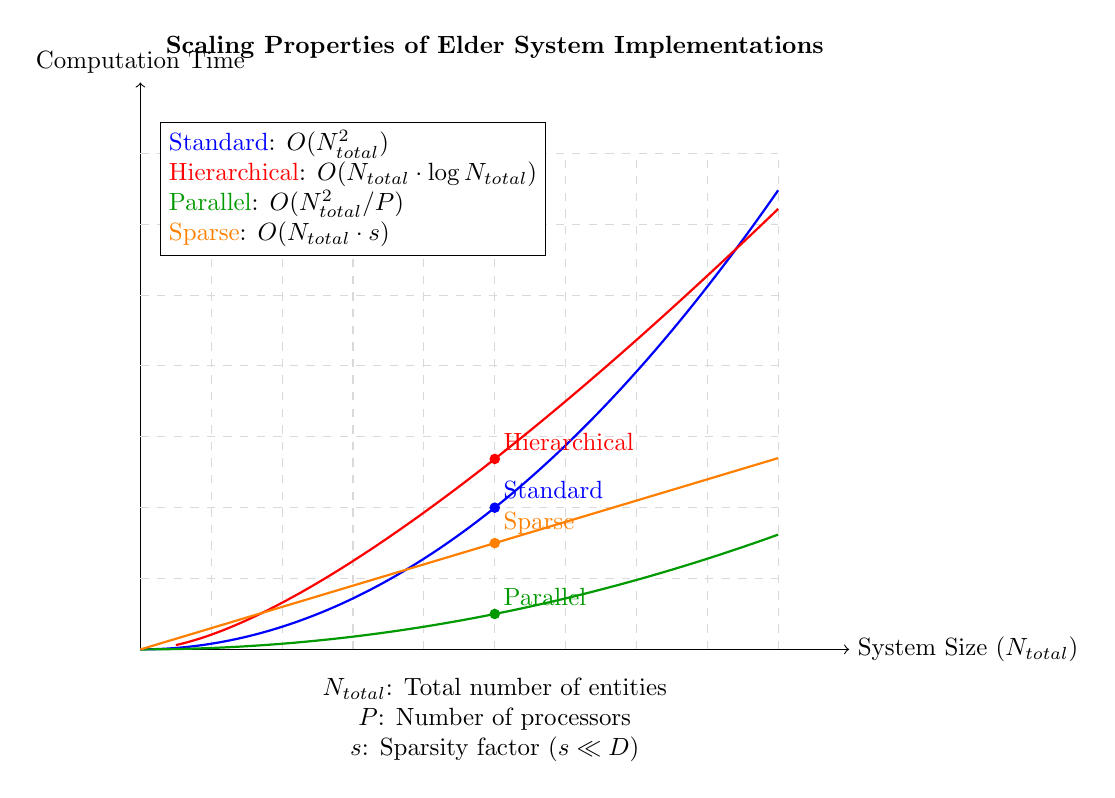
\begin{tikzpicture}[scale=0.9, transform shape]
    % Define styles
    \tikzset{
        axistitle/.style={font=\bfseries},
        gridline/.style={gray!30, dashed},
        legendbox/.style={draw, fill=white, align=left},
        standard/.style={blue, thick},
        hierarchical/.style={red, thick},
        parallel/.style={green!60!black, thick},
        sparse/.style={orange, thick}
    }
    
    % Draw coordinate system
    \draw[->] (0,0) -- (10,0) node[right] {System Size ($N_{total}$)};
    \draw[->] (0,0) -- (0,8) node[above] {Computation Time};
    
    % Add grid
    \foreach \x in {1,2,...,9}
        \draw[gridline] (\x,0) -- (\x,7);
    \foreach \y in {1,2,...,7}
        \draw[gridline] (0,\y) -- (9,\y);
    
    % Plot curves
    % Standard implementation: O(N²)
    \draw[standard] plot[domain=0:9, samples=100] (\x, {min(7, 0.08*\x*\x)});
    
    % Hierarchical optimization: O(N·log N)
    \draw[hierarchical] plot[domain=0.5:9, samples=100] (\x, {min(7, 0.3*\x*ln(\x+1))});
    
    % Parallel implementation: O(N²/P)
    \draw[parallel] plot[domain=0:9, samples=100] (\x, {min(7, 0.08*\x*\x/4)});
    
    % Sparse implementation: O(N·s)
    \draw[sparse] plot[domain=0:9, samples=100] (\x, {min(7, 0.3*\x)});
    
    % Add key points
    \node[circle, fill=blue, inner sep=1.5pt] at (5, {0.08*5*5}) {};
    \node[above right, blue] at (5, {0.08*5*5}) {Standard};
    
    \node[circle, fill=red, inner sep=1.5pt] at (5, {0.3*5*ln(5+1)}) {};
    \node[above right, red] at (5, {0.3*5*ln(5+1)}) {Hierarchical};
    
    \node[circle, fill=green!60!black, inner sep=1.5pt] at (5, {0.08*5*5/4}) {};
    \node[above right, green!60!black] at (5, {0.08*5*5/4}) {Parallel};
    
    \node[circle, fill=orange, inner sep=1.5pt] at (5, {0.3*5}) {};
    \node[above right, orange] at (5, {0.3*5}) {Sparse};
    
    % Add legend
    \node[legendbox] at (3,6.5) {
        \textcolor{blue}{Standard}: $O(N_{total}^2)$\\
        \textcolor{red}{Hierarchical}: $O(N_{total} \cdot \log N_{total})$\\
        \textcolor{green!60!black}{Parallel}: $O(N_{total}^2 / P)$\\
        \textcolor{orange}{Sparse}: $O(N_{total} \cdot s)$
    };
    
    % Add annotations
    \node[align=center] at (5,-1) {
        $N_{total}$: Total number of entities\\
        $P$: Number of processors\\
        $s$: Sparsity factor ($s \ll D$)
    };
    
    % Add title
    \node[axistitle] at (5,8.5) {Scaling Properties of Elder System Implementations};
    
\end{tikzpicture}
\caption{Scaling properties of different Elder system implementations as a function of system size ($N_{total}$). The standard implementation scales quadratically due to orbital dynamics calculations. Hierarchical optimizations reduce this to $O(N_{total} \cdot \log N_{total})$ by leveraging the hierarchical structure. Parallel implementations divide the work across $P$ processors, providing linear speedup. Sparse implementations take advantage of sparse connectivity, achieving linear scaling with a small constant factor $s$.}
\label{fig:scaling_properties}
\end{figure}